\documentclass{beamer}
\usepackage{pgfpages}

% \setbeameroption{show notes}
% \setbeameroption{show notes on second screen=right}
\usepackage[T1]{fontenc}
\usepackage{libertine}
\renewcommand*\ttdefault{txtt}

\usepackage{adjustbox}
\usepackage{algorithm}
\usepackage{algpseudocode}
\usepackage{array}
\usepackage{booktabs}
\usepackage[center]{caption}
\usepackage{color}
\usepackage{graphicx}
\usepackage{mathtools}
\usepackage{rnamacros}
\usepackage{tabularx}
\usepackage{xspace}

\captionsetup[figure]{labelformat=empty}
\definecolor{litegray}{gray}{0.75}
\graphicspath{{Images/}}
\usefonttheme{professionalfonts}
\setbeamerfont{caption}{size=\tiny}
\setbeamercovered{transparent}

\newcommand{\slidefigure}[2][1]{\includegraphics[width=#1\textwidth,height=#1\textheight,keepaspectratio]{#2}}
\newcommand{\btVFill}{\vskip 0pt plus 1filll}

\title[Coarse-Grained RNA Folding Kinetics]{On the Use of Coarse-Grained Thermodynamic Landscapes to Efficiently Estimate Folding Kinetics for RNA Molecules}
\author{Evan Senter}
\date{2015}

\AtBeginSection[] {
\begin{frame}
	<beamer>{Outline}
	\tableofcontents[currentsection]
\end{frame}
}

\begin{document}

\frame{\titlepage}

\section{Overview}

\begin{frame}
	\frametitle{About me}
	\begin{columns}
		\column{.55\textwidth}
		\begin{block}
			{My background}
			\begin{itemize}
				\item B.A. in Computer Science, Computational Biology
				\item Worked in software engineering for $\approx$ 2 years after
				\item Started at Boston College in Fall, 2011
				\item Joined the Clote Lab focusing on Computational RNA Biology
			\end{itemize}
		\end{block}

		\column{.45\textwidth}
		\begin{figure}
			\centering \slidefigure{ucsb} \caption{University of California, Santa Barbara}
		\end{figure}
	\end{columns}
\end{frame}

\begin{frame}
	\frametitle{Goal of this talk}
	\begin{block}
		{Primary aim} Present research on rapidly estimating RNA folding kinetics {\em in silico}
	\end{block}
	\begin{enumerate}
		\item Motivate interest in the study of RNA
		\item Highlight interesting roles of non-coding RNAs (ncRNA)
		\item Identify biological relevance of folding kinetics
		\item Present overview of findings
		\item Explain research leading to these findings
	\end{enumerate}
\end{frame}

\begin{frame}
	\frametitle{What's the takeaway?}
	\begin{itemize}
		\pause
		\item A thesis?\dots
	\end{itemize}
\end{frame}

\begin{frame}
	\frametitle{How biologists See bioinfor{\em magicians}}
	\begin{figure}
		\centering \slidefigure{nemo}
	\end{figure}
\end{frame}

\begin{frame}
	\frametitle{A biologist when stumbling into a math-heavy talk\dots}
	\begin{figure}
		\centering \slidefigure{nemofocus}
	\end{figure}
\end{frame}

\begin{frame}
	\frametitle{What we aim for\dots}
	\begin{figure}
		\centering \slidefigure{nemoturtle}
	\end{figure}
\end{frame}

\section{Background}

\begin{frame}
	\frametitle{Why do we care about RNA?}
	\begin{columns}
		\column{.55\textwidth}
		\begin{itemize}
			\item<1-> Phrase `junk DNA' pigeonholed RNA into predetermined roles
			\begin{itemize}
				\item<2-> Messenger RNA (mRNA)
				\item<2-> Transfer RNA (tRNA)
				\item<2-> Ribosomal RNA (rRNA)
			\end{itemize}
			\item<3-> Diverse roles for ncRNA beyond rRNA and tRNA
		\end{itemize}

		\column{.45\textwidth}
		\begin{figure}
			\centering \slidefigure{crick1970} \caption{Crick, F. (1970). Central dogma of molecular biology. Nature.}
		\end{figure}
	\end{columns}
\end{frame}

\begin{frame}
	\frametitle{ncRNAs---what are they good for?}
	\begin{block}
		{The reality} We were not wrong in assigning importance to the aforementioned roles of RNA, but\dots
	\end{block}
\end{frame}

\begin{frame}
	\frametitle{ncRNAs---what are they good for?}

	We have since found a diverse set of roles for RNA, including\dots
  \pause
	\begin{itemize}
		\item<2-> Peptide bond catalysis
		\item[]<2-> \scriptsize Nissen, P., Hansen, J., Ban, N., Moore, P. B., \& Steitz, T. A. (2000). The structural basis of ribosome activity in peptide bond synthesis. Science (New York, N.Y.), 289(5481), 920--930.

		% No protein side-chain within 18 angstroms of catalytic cite of peptide bond formation, indicating ribosomal RNA is a ribozyme

		\item<3-> Intron splicing
		\item[]<3-> \scriptsize Cate, J. H., Gooding, A. R., Podell, E., Zhou, K., Golden, B. L., Kundrot, C. E., et al. (1996). Crystal structure of a group I ribozyme domain: principles of RNA packing. Science (New York, N.Y.), 273(5282), 1678--1685.
		\item<4-> Post-transcriptional gene regulation via RNAi
		\item[]<4-> \scriptsize Fire, A., Xu, S., Montgomery, M. K., Kostas, S. A., Driver, S. E., \& Mello, C. C. (1998). Potent and specific genetic interference by double-stranded RNA in Caenorhabditis elegans. Nature, 391(6669), 806--811.
		\item[]<4->
	\end{itemize}
\end{frame}

\begin{frame}
	\frametitle{ncRNAs---what are they good for?}
	\begin{itemize}
		\item<1-> Xist ncRNA for suppression of inactive X chromosome
		\item[]<1-> \scriptsize Penny, G. D., Kay, G. F., Sheardown, S. A., Rastan, S., \& Brockdorff, N. (1996). Requirement for Xist in X chromosome inactivation. Nature, 379(6561), 131--137.
		\item<2-> Retranslation events (SECIS elements)
		\item[]<2-> \scriptsize Walczak, R., Westhof, E., Carbon, P., \& Krol, A. (1996). A novel RNA structural motif in the selenocysteine insertion element of eukaryotic selenoprotein mRNAs. Rna, 2(4), 367--379.

		% Selenocysteine insertion sequences located in 3' UTR that cause re-translation of UGA stop codon as selenocysteine

		\item<3-> Ribosomal frameshift events
		\item[]<3-> \scriptsize Jacks, T., Power, M. D., Masiarz, F. R., Luciw, P. A., Barr, P. J., \& Varmus, H. E. (1988). Characterization of ribosomal frameshifting in HIV-1 gag-pol expression. Nature, 331(6153), 280--283.
		\item[]<3-> \scriptsize Ofori, L. O., Hilimire, T. A., Bennett, R. P., Brown, N. W., Smith, H. C., \& Miller, B. L. (2014). High-affinity recognition of HIV-1 frameshift-stimulating RNA alters frameshifting in vitro and interferes with HIV-1 infectivity. Journal of Medicinal Chemistry, 57(3), 723--732.

		% gag-pol frameshift frequency (5% efficiency) required to maintain balance of Gag to Gag-Pol protein ratio

		\item[]<3->
	\end{itemize}
\end{frame}

\begin{frame}
	\frametitle{ncRNAs---what are they good for?}

	And finally\dots
	\begin{itemize}
		\item<1-> Transcriptional and translational regulation via riboswitches
		\item[]<1-> \scriptsize Nahvi, A., Sudarsan, N., Ebert, M. S., Zou, X., Brown, K. L., \& Breaker, R. R. (2002). Genetic Control by a Metabolite Binding mRNA. Chemistry \& Biology, 9(9), 1043--1049.
		\item<2-> Spliced leader (SL) trans-splicing events in {\em L. collosoma}
		\item[]<2-> \scriptsize LeCuyer, K. A., \& Crothers, D. M. (1993). The {\em Leptomonas collosoma} spliced leader RNA can switch between two alternate structural forms. Biochemistry, 32(20), 5301--5311.
		\item<3-> hok/sok postsegregational killing mechanism in {\em E. coli}
		\item[]<3-> \scriptsize Gerdes, K., Rasmussen, P. B., \& Molin, S. (1986). Unique type of plasmid maintenance function: postsegregational killing of plasmid-free cells. Proceedings of the National Academy of Sciences, 83(10), 3116--3120.
		\item[]<3-> \scriptsize Nagel, J. H., Gultyaev, A. P., Gerdes, K., \& Pleij, C. W. (1999). Metastable structures and refolding kinetics in hok mRNA of plasmid R1. Rna, 5(11), 1408--1418.
		\item[]<3->
	\end{itemize}
\end{frame}

\begin{frame}
	\frametitle{ncRNAs---what are they good for?}
	\begin{block}
		{Summary} ncRNAs have diverse cellular responsibilities, beyond the canonical tRNA and rRNA examples
	\end{block}
\end{frame}

% Hopefully these breif examples have helped to establish the diverse cellular roles that ncRNAs are responsible for.

\begin{frame}
	\frametitle{{\em hok/sok} and kinetics}
	\begin{columns}
		\column{.5\textwidth}
		\begin{figure}
			\centering \slidefigure{r1present}
		\end{figure}

		\column{.5\textwidth}
		\begin{figure}
			\centering \slidefigure{r1missing}
		\end{figure}
	\end{columns}

	\btVFill
	\begin{center}
		\tiny \color{litegray} \url{https://en.wikipedia.org/wiki/File:Hok_sok_system_R1_plasmid_present.gif} \\
		\url{https://en.wikipedia.org/wiki/File:Hok_sok_system_R1_plasmid_absent.gif}
	\end{center}
\end{frame}

\begin{frame}
	\frametitle{{\em hok/sok} structures}
	\begin{figure}
		\centering \slidefigure{hoksoksequence} \caption{Adapted from Thisted, T., \& Gerdes, K. (1992). Mechanism of post-segregational killing by the {\em hok}/{\em sok} system of plasmid R1. Sok antisense RNA regulates {\em hok} gene expression indirectly through the overlapping {\em mok} gene. Journal of Molecular Biology, 223(1), 41--54.}
	\end{figure}
\end{frame}

\begin{frame}
	\frametitle{{\em hok} folding kinetics}
	\begin{columns}
		\column{.65\textwidth}
		\begin{figure}
			\centering \slidefigure[.7]{hoktranscription} \caption{\tiny Adapted from Nagel, J. H., Gultyaev, A. P., Gerdes, K., \& Pleij, C. W. (1999). Metastable structures and refolding kinetics in hok mRNA of plasmid R1. RNA, 5(11), 1408--1418.}
		\end{figure}

		\column{.35\textwidth}
		\begin{figure}
			\centering \slidefigure{hokrefoldingkinetics} \caption{\tiny Nagel, J. H. A., Gultyaev, A. P., Oist{\"a}m{\"o}, K. J., Gerdes, K., \& Pleij, C. W. A. (2002). A pH-jump approach for investigating secondary structure refolding kinetics in RNA. Nucleic Acids Research, 30(13), e63.}
		\end{figure}
	\end{columns}
\end{frame}

\begin{frame}
  \frametitle{How are RNA kinetics experimentally measured?}

  \begin{block}
    {Experimental protocols include\dots}
    \begin{itemize}
      \item<1-> Temperature-jump experiments
      \item[]<1-> \scriptsize Cole, P. E., \& Crothers, D. M. (1972). Conformational changes of transfer ribonucleic acid. Relaxation kinetics of the early melting transition of methionine transfer ribonucleic acid ({\em Escherichia coli}). Biochemistry, 11(23), 4368--4374.
      \item<2-> pH-jump experiments
      \item[]<2-> \scriptsize Bina-Stein, M., \& Crothers, D. M. (1974). Conformational changes of transfer ribonucleic acid. The pH phase diagram under acidic conditions. Biochemistry, 13(13), 2771--2775.
      \item<3-> Single molecule mechanical tension
      \item[]<3-> \scriptsize Vieregg, J. R., \& Tinoco, I. (2006). Modelling RNA folding under mechanical tension. Molecular Physics, 104(8), 1343--1352.
      \item<4-> Fluorescence resonance energy transfer (FRET)
      \item[]<4-> \scriptsize Zhuang, X., \& Rief, M. (2003). Single-molecule folding. Current Opinion in Structural Biology, 13(1), 88--97.
      \item[]<4->
    \end{itemize}
  \end{block}
\end{frame}

\begin{frame}
	\frametitle{Organization of Hermes}
	\begin{figure}
		\centering \slidefigure{Figures/Hermes/softwareOrg}
	\end{figure}
\end{frame}

% All have something in common. Conservation of secondary structure across those motifs performing similar function, introducing
% the idea of families of RNA with similar function, grouped in large part by a common secondary structure.
% Define secondary structure, how it's more important for RNA than proteins and there exists a finite number of conformations.
% Griffiths-Jones, S., Bateman, A., Marshall, M., Khanna, A., \& Eddy, S. R. (2003). Rfam: an RNA family database. Nucleic Acids Research, 31(1), 439--441.
% Mean first passage time and Kevin Bacon
% Two questions, 1) what's the fewest number of friends you have to go to before you get to Kevin Bacon, and what is the average number?
% Temperature jump experiments, FRET, single molecule mechanical tension

\begin{frame}
	\frametitle{Comparison of various kinetics programs}
  \resizebox{\linewidth}{!}{
    \centering
  	\begin{tabular}
  		{*{9}{l}} \toprule \small{Hastings (Yes\textbackslash No)} & \small{\rnamfpt} & \small{\rnaeq} & \small{\kinfold} & \small{\fftmfpt} & \small{\rnatwofold} & \small{\fftbor} & \small{\barrierseq} & \small{\ffteq} \\
  		\cmidrule(l){2-9}
  		% rnamfpt rnaeq kinfold fftmfpt rnatwofold fftbor barrierseq ffteq
  		\small{\rnamfpt} & $1$ & $0.5683$ & \textcolor{red}{$0.7945$} & \textcolor{red}{$0.5060$} & $0.5110$ & $0.5204$ & $0.5280$ & $0.4472$ \\
  		\small{\rnaeq} & $0.5798$ & $1$ & $0.7814$ & $0.7043$ & $0.7025$ & $0.5080$ & \textcolor{blue}{$0.5979$} & \textcolor{blue}{$0.6820$} \\
  		\small{\kinfold} & \textcolor{red}{\textbf{$0.7933$}} & $0.7507$ & $1$ & \textcolor{red}{$0.7312$} & $0.7358$ & $0.6241$ & $0.6328$ & $0.6445$ \\
  		\small{\fftmfpt} & \textcolor{red}{\textbf{$0.6035$}} & $0.7935$ & \textcolor{red}{$0.7608$} & $1$ & $0.9980$ & $0.5485$ & $0.8614$ & $0.9589$ \\
  		\small{\rnatwofold} & $0.6076$ & $0.7919$ & $0.7655$ & $0.9983$ & $1$ & $0.5584$ & $0.8538$ & $0.9515$ \\
  		\small{\fftbor} & $0.5416$ & $0.5218$ & $0.6241$ & $0.5748$ & $0.5855$ & $1$ & $0.3450$ & $0.4229$ \\
  		\small{\barrierseq} & $0.6346$ & \textcolor{blue}{$0.6578$} & $0.6328$ & $0.8310$ & $0.8217$ & $0.3450$ & $1$ & \textcolor{blue}{$0.9149$} \\
  		\small{\ffteq} & $0.5614$ & \textcolor{blue}{$0.7916$} & $0.6966$ & $0.9670$ & $0.9590$ & $0.4757$ & \textcolor{blue}{$0.8940$} & $1$ \\
  		\bottomrule
  	\end{tabular}
	} \vspace{2em}
	\begin{itemize}
		\scriptsize
		\item \rnamfpt, \fftmfpt, \rnaeq, and \ffteq included in the \hermes package
		\item \rnatwofold (Lorenz {\em et. al.}, 2009), \barrierseq (Flamm {\em et. al.}, 2002), and \fftbor (Senter {\em et. al.}, 2012) kinetics computed with \hermes
	\end{itemize}
\end{frame}

\begin{frame}
  \frametitle{RNA representation}
  \begin{block}
    {Sequence} An RNA sequence is a string $\seq = \seqN$, where $s_i \in \{\text{A,\,U,\,G,\,C}\}$
  \end{block}
  \begin{block}
    {Structure} An secondary structure \str compatible with \seq is a collection of base pair tuples such $(i,j)$, such that:
    \begin{itemize}
      \item $(\seq_i, \seq_j) \in \bpSet$
      \item $1 \le i \le i+\theta < j \le n$ where $\theta \ge 0$
      \item Given $(i,j), (x,y)$ from \str, $i=x \iff j=y$
      \item Given $(i,j), (x,y)$ from \str, $i<x<j \iff i<y<j$
    \end{itemize}
  \end{block}
  \begin{align*}
    \bpSet = \{\text{(A,\,U),\,(U,\,A),\,(G,\,C),\,(C,\,G),\,(G,\,U),\,(U,\,G)}\}
  \end{align*}
\end{frame}

\begin{frame}
  \frametitle{Structural motifs}
  \begin{columns}
    \column{.65\textwidth}
    \begin{figure}
      \centering
      \slidefigure{rnass}
      \caption{Lu, X.-J., Bussemaker, H. J., \& Olson, W. K. (2015). DSSR: an integrated software tool for dissecting the spatial structure of RNA. Nucleic Acids Research.}
    \end{figure}

    \column{.35\textwidth}
    \begin{block}
      {Structural Motifs}
      \begin{enumerate}
        \item Exterior loop
        \item Stack
        \item Interior loop
        \item Multiloop
        \item Bulge
        \item Hairpin
      \end{enumerate}
    \end{block}
  \end{columns}
\end{frame}

\begin{frame}
  \frametitle{Base pair distance}
  \begin{block}
    {Symmetric distance}
    \begin{align*}
      \dBP{\str}{\strT} = |\str \cup \strT| - |\str \cap \strT|
    \end{align*}
  \end{block}
  \begin{block}
    {Distance between two structures}
    \begin{align*}
      \begin{split}
        \dBP{\str_{[i,j]}}{\strT_{[i,j]}} &= |\{ (x,y): i \leq x<y\leq j, \\
        & (x,y) \in \str - \strT \text{ or } (x,y) \in \strT - \str \}| = k
      \end{split}
    \end{align*}
  \end{block}
\end{frame}

\begin{frame}
	\frametitle{Performance characteristics}
	\begin{columns}
		\column{.5\textwidth}
		\begin{figure}
      \includegraphics[width=\linewidth]{Figures/FFTbor2D/ffttwoRtwofoldTiming}
      \caption{\ffttwo vs. \rnatwofold benchmarking}
    \end{figure}

		\column{.5\textwidth}
    \begin{figure}
      \includegraphics[width=\linewidth]{Figures/FFTbor2D/ffttwoRtwofoldLogScale}
      \caption{\ffttwo vs. \rnatwofold benchmarking (log scale)}
    \end{figure}
	\end{columns}
\end{frame}

\begin{frame}
	\frametitle{Performance characteristics}
	\begin{columns}
		\column{.5\textwidth}
		\includegraphics[width=\linewidth]{Figures/FFTbor2D/ffttwoRtwofoldStdev}

		\column{.5\textwidth}
		\begin{itemize}
			\item Approach using FFT goes from \On{7} to \On{5}
			\item We observe a real performance gain in line with 100x speedup
			\item Memory requirements drop from \On{4} to \On{2}
			\item More consistent performance characteristics
		\end{itemize}
	\end{columns}
\end{frame}

\begin{frame}
	\frametitle{And of course my labmates and fellow grad students!}
	\begin{figure}
		\centering
		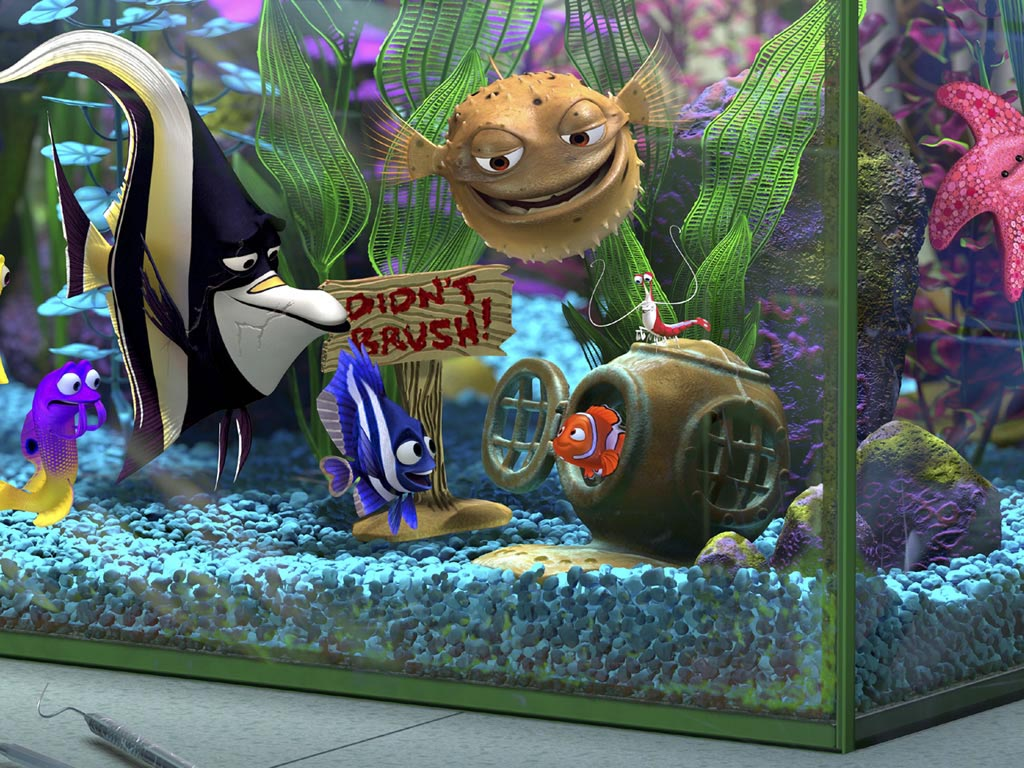
\includegraphics[width=\linewidth]{labmates}
	\end{figure}
\end{frame}

\begin{frame}
	\frametitle{Questions?}
	\begin{figure}
		\centering
		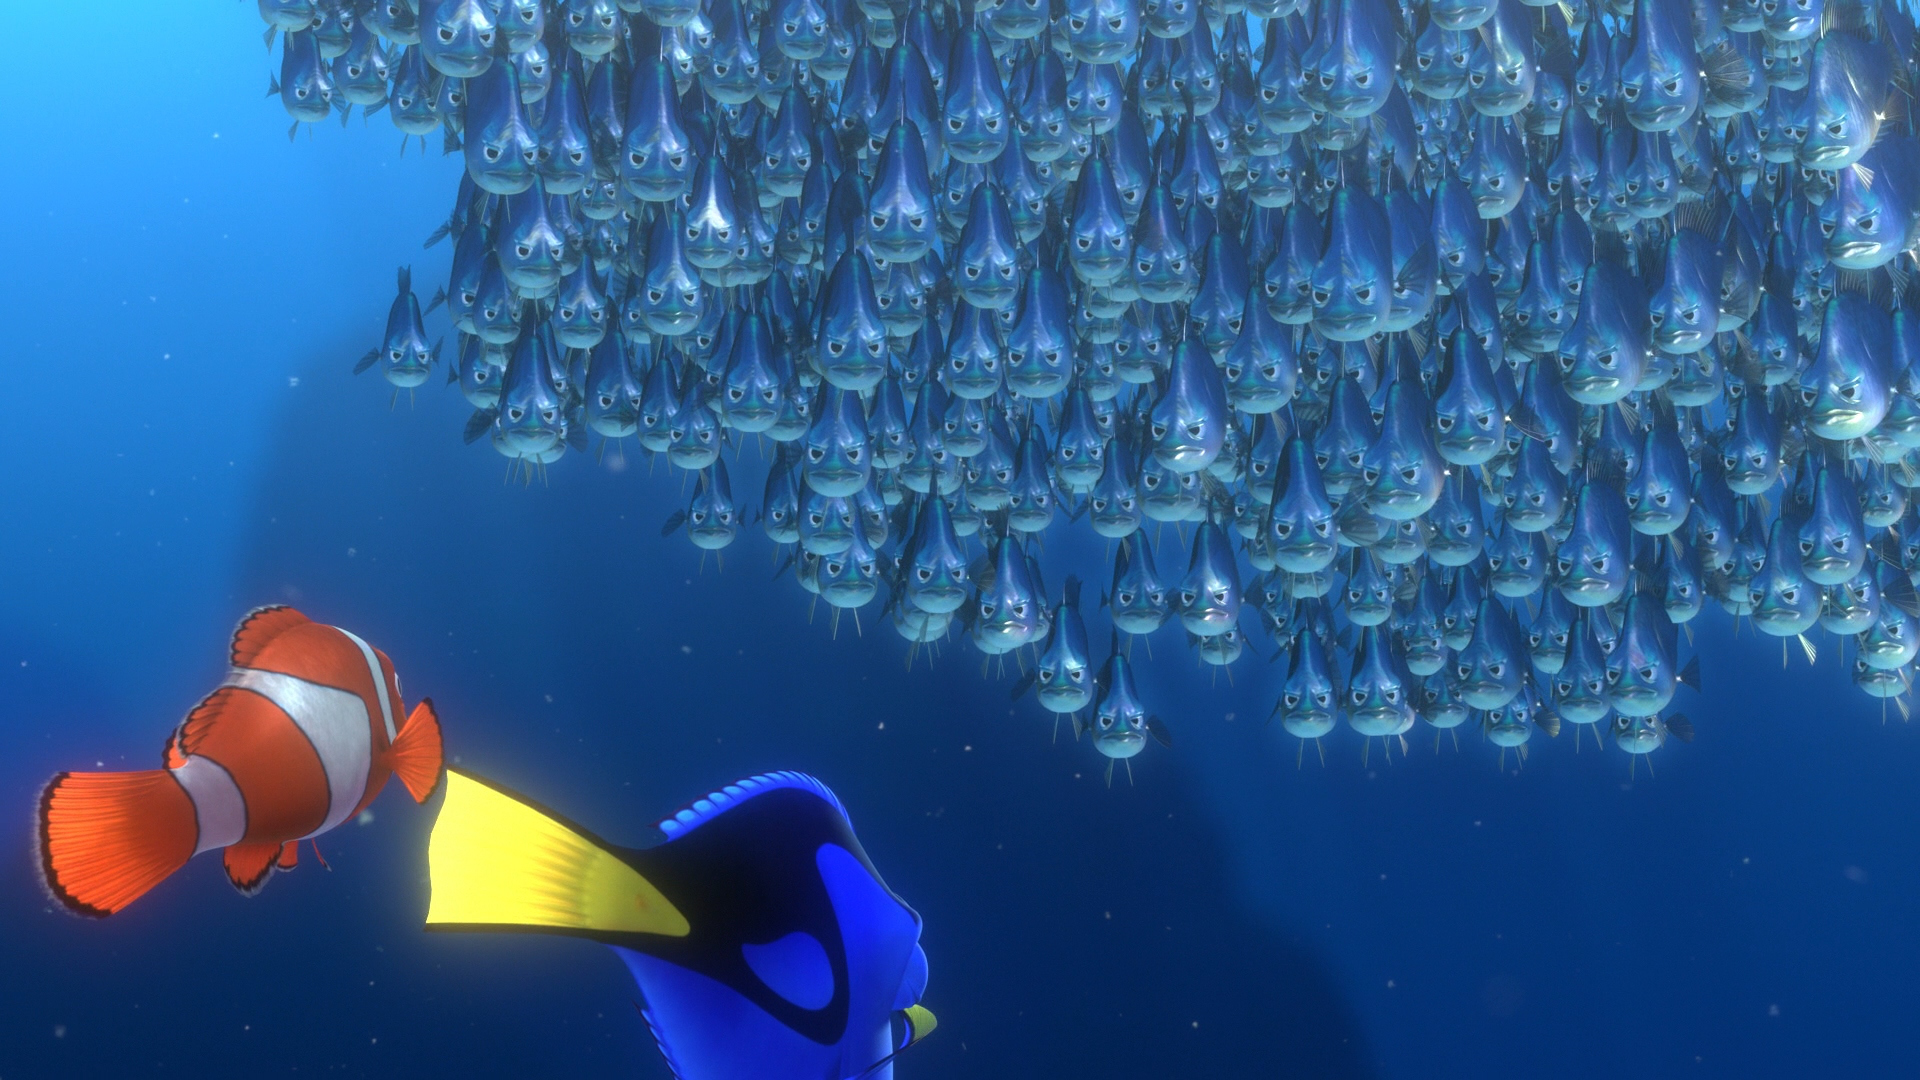
\includegraphics[width=\linewidth]{questions}
	\end{figure}
\end{frame}

\section{Problem definition}

\begin{frame}
	\frametitle{Problem Definition}
	\begin{block}
		{Desire} Given an input sequence \seq and two input structures \strA, \strB, we would like to compute \alert{all} possible structures \strS compatible with \seq, and bin them into discrete sets based on their {\em distance} to \strA and \strB
	\end{block}
	\begin{alertblock}
		{Issue} Consider $\mathbb{S}$ to be the set of all structures compatible with \seq. It has been shown that $|\mathbb{S}|$ grows exponentially with sequence length $n$
	\end{alertblock}
	\begin{block}
		{Refinement} Rather than store $\mathbb{S}$ at any point in time, we will use dynamic programming to compute the thermodynamic properties of these bins
	\end{block}
\end{frame}

\begin{frame}
	\frametitle{Parameterized Partition Function, 1D}
	\begin{block}
		{\bfZ{}{} binned by $k$}
		\begin{align*}
			\bfZ{k}{} = \bfZ{k}{1,n} = \sum_{\mathclap{\substack{\str \text{ such that }\rule[-.5ex]{0pt}{0pt} \\
			\dBP{\str}{\strSt}=k}}}\; \boltzF{\str}
		\end{align*}
	\end{block}
\end{frame}

\begin{frame}
	\frametitle{Recursions to compute \bfZ{k}{i,j}}
	\begin{block}
		{Structural decomposition from one target}
		\begin{align*}
			\bfZ{k}{i,j} = \bfZ{k-b_0}{i,j-1}\enspace + \sum_{\substack{s_r s_j \in \bpSet, \\
			i \le r<j}} \left( \boltzNuss{r,j}\enspace \sum_{\mathclap{w+w'=k-b(r)}}\quad \bfZ{w}{i,r-1} \bfZ{w'}{r+1,j-1} \right)
		\end{align*}
	\end{block}
\end{frame}

\begin{frame}
	\frametitle{Parameterized Partition Function, 2D}
	\begin{block}
		{\bfZ{}{} binned by $x,y$ pairs}
		\begin{align*}
			\bfZ{x,y}{1,n}\;=\; \sum_{\mathclap{\substack{ \str \text{ such that } \rule[-.5ex]{0pt}{0pt} \\
			\dBP{\str}{\strA} = x,\,\dBP{\str}{\strB} = y}}}\enspace \boltzF{\str}
		\end{align*}
	\end{block}
\end{frame}

\begin{frame}
	\frametitle{Recursions to compute \bfZ{x,y}{i,j}}
	\begin{block}
		{Structural decomposition from two targets}
		\begin{align*}
			\begin{split}
				& \bfZ{x,y}{i,j} = \bfZ{x- \omega_0,y-\beta_0}{i,j-1}\enspace + \\
				& \sum_{\substack{s_k s_j \in \bpSet, \\
				i \le k<j}} \left( \boltzNuss{k,j}\quad \sum_{\mathclap{u+u'=x- \omega(k)}}\hspace{3.75em} \sum_{\mathclap{v+v'=y-\beta(k)}}\quad \bfZ{u,v}{i,k-1} \cdot \bfZ{u',v'}{k+1,j-1} \right)
			\end{split}
		\end{align*}
	\end{block}
\end{frame}

\begin{frame}
	\frametitle{Partition function of a variable $x$}
	\begin{block}
		{Only compute \emZ{i,j}{x} instead of \bfZ{x,y}{i,j}}
		\begin{align*}
			\begin{split}
				& \emZ{i,j} = \emZof{i,j-1}{x} \cdot x^{ \omega_0n+\beta_0} + \\
				&\sum_{\substack{s_k s_j \in \bpSet,\\i\le k<j}} \left(e^{\frac{-E_0(k,j)}{RT}}\cdot \emZof{i,k-1}{x} \cdot \emZof{k+1,j-1}{x}\cdot x^{ \omega(k)n+\beta(k)} \right)
			\end{split}
		\end{align*}
	\end{block}
\end{frame}

\begin{frame}
	\frametitle{FFT background}
	\begin{block}
		{Complex {\em k}th roots of unity}
		\begin{align*}
			\omega_0=\exp(\frac{0\cdot 2\pi i}{n^2}), \omega_1=\exp(\frac{1\cdot 2\pi i}{n^2}),\dots, \omega_{n^2-1}=\exp(\frac{(n^2-1)\cdot 2\pi i}{n^2})
		\end{align*}
	\end{block}
	\begin{block}
		{Evaluate \emZ{i,j}{x} for all $n^2$ roots of unity}
		\begin{align*}
			y_0=\emZof{}{ \omega_0},\dots,y_{n^2-1}=\emZof{}{ \omega_{n^2-1}})
		\end{align*}
	\end{block}
	\begin{block}
		{Represent results of evaluation in column form}
		\begin{align*}
			\bfY = (y_0,\dots,y_{n^2-1})^{\text T}
		\end{align*}
	\end{block}
\end{frame}

\begin{frame}
	\frametitle{Vandermonde matrix}
	\begin{block}
		{Matrix construction}
		\begin{align*}
			V_{n} = \left(
			\begin{array}{rrrrr}
				1 & 1 & 1 & \dots & 1 \\
				1 & \omega & \omega^2 & \dots & \omega^{n-1} \\
				1 & \omega^2 & \omega^4 & \dots & \omega^{2(n-1)} \\
				1 & \omega^3 & \omega^6 & \dots & \omega^{3(n-1)} \\
				\vdots & \vdots & \vdots & \vdots & \vdots \\
				1 & \omega^{n-1} & \omega^{2(n-1)} & \dots & \omega^{(n-1)(n-1)} \\
			\end{array}
			\right)
		\end{align*}
	\end{block}
\end{frame}

\begin{frame}
	\begin{definition}
		Define the FFT to be the $O(n \log n)$ algorithm to compute the Discrete Fourier Transform (DFT), defined as the matrix product $\bfY = V_{n} {\bf A}$
	\end{definition}
	\begin{align*}
		\left(
		\begin{array}{l}
			y_0 \\
			y_1 \\
			y_2 \\
			\vdots \\
			y_{n^2-1} \\
		\end{array}
		\right) = V_n \cdot \left(
		\begin{array}{l}
			a_0 \\
			a_1 \\
			a_2 \\
			\vdots \\
			a_{n^2-1} \\
		\end{array}
		\right)
	\end{align*}
\end{frame}

\begin{frame}
	Since we defined $\bfY = (y_0,\dots,y_{n-1})^{\text T}$, where:
	\begin{align*}
		y_0=\emZof{}{\omega_0},\dots,y_{n^2-1}=\emZof{}{\omega{n^2-1}})
	\end{align*}

	and $\omega_k = \exp(\frac{2\pi ki}{n^2})$, it follows that the coefficients $c_{rn+s}=\bfZ{rn+s}{1,n}$ in the polynomial:
	\begin{align*}
		\emZ{} = c_0 + c_1 x + \dots + c_{n^2-1} x^{n^2-1}
	\end{align*}

	can be computed using the \fft, and:
	\begin{align*}
		c_{rn+s}=\;=\; \sum_{\mathclap{\substack{ \str \text{ such that } \rule[-.5ex]{0pt}{0pt} \\
		\dBP{\str}{\strA} = r,\,\dBP{\str}{\strB} = s}}}\enspace \boltzF{\str}
	\end{align*}
\end{frame}

\end{document}
